%=========================================================
\chapter{Modelo dinámico}	
\label{cap:modDinamico}

	Este capítulo describe en modelo dinámico del sistema. en el se detallan todos los escenarios de ejecución del sistema. La figura~\ref{fig:casosDeUso} muestra el diagrama general del sistema y sus sib sistemas, y la figura~\ref{fig:casosDeUsoDetalle} muestra todos los casos de uso del sistema. En este documento solo detallamos los casos de uso del subsistema de gestión de cursos.
	
\begin{figure}[htbp]
	\begin{center}
		\fbox{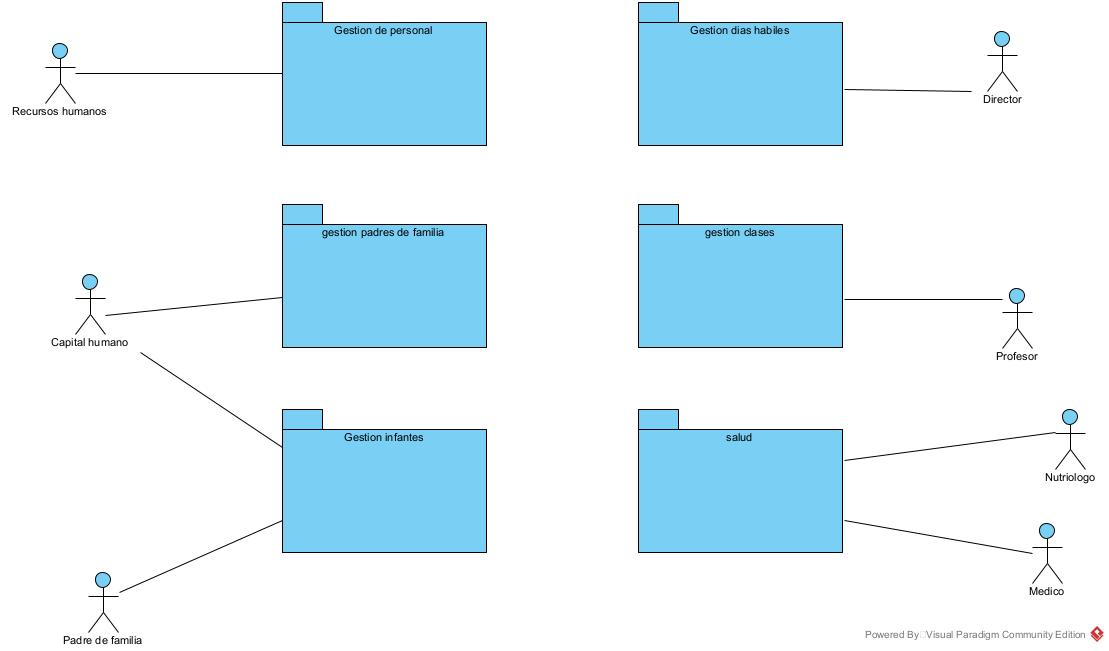
\includegraphics[width=.8\textwidth]{images/casosDeUso}}
		\caption{Diagrama de casos de uso del sistema.}
		\label{fig:casosDeUso}
	\end{center}
\end{figure}

\begin{figure}[htbp]
	\begin{center}
		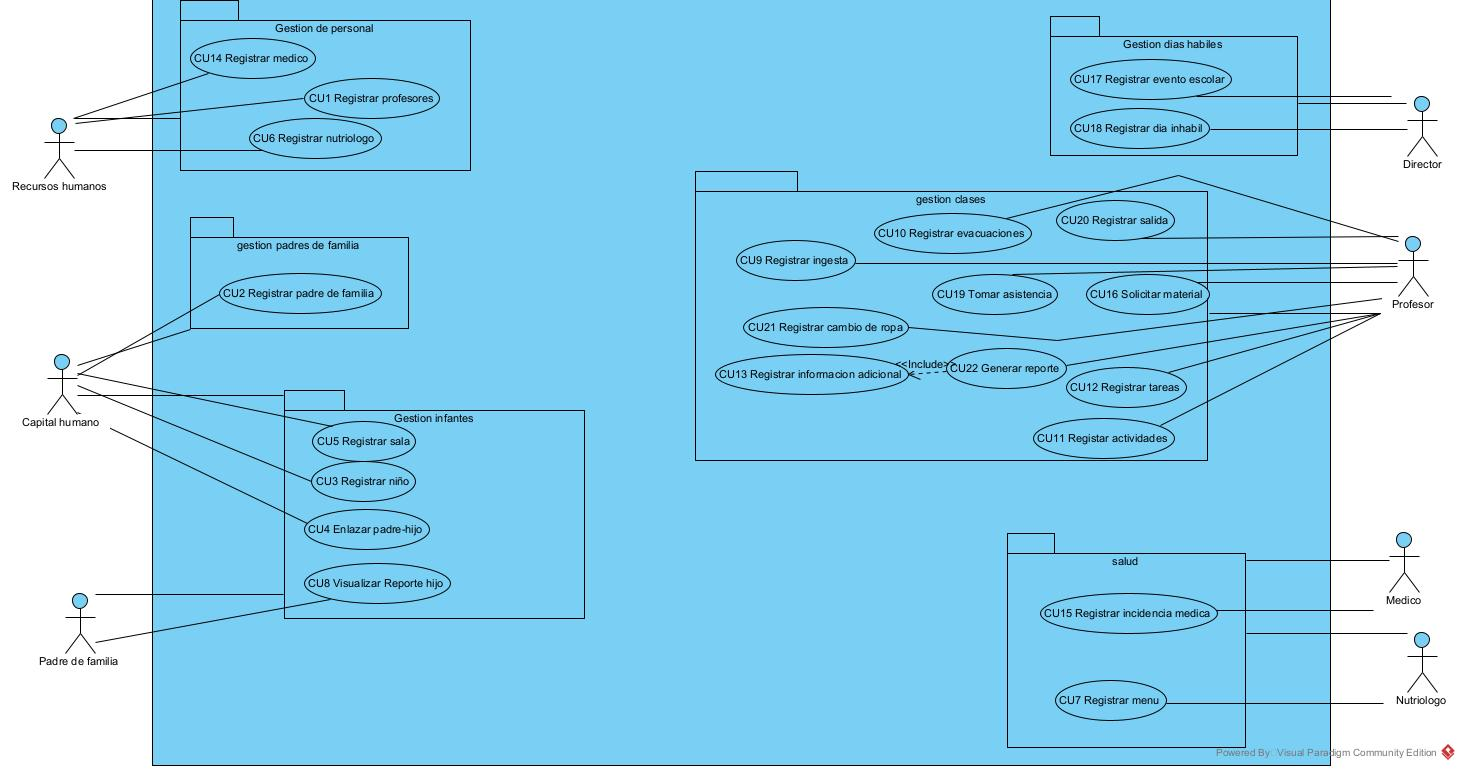
\includegraphics[angle=90, width=.7\textwidth]{images/casosDeUsoDetalle}
		\caption{Diagrama detallado del sistema.}
		\label{fig:casosDeUsoDetalle}
	\end{center}
\end{figure}

%---------------------------------------------------------
\section{Descripción de actores}

%---------------------------------------------------------
\begin{Usuario}{\hypertarget{recursosHumanos}{\subsection{Recursos humanos}}}{
	Es el responsable de la gestion del personal dentro de la guarderia.
}
    \item[Responsabilidades:] \cdtEmpty
    \begin{itemize}
		\item Administrar la contratacion y despido del personal
		
    \end{itemize}

	\item[Perfil:] \cdtEmpty
    \begin{itemize}
		\item Licenciatura en recursos humanos, administracion de empresas o afin.
		\item un año de experiencia minimo en gestion de recursos humanos.
		\item Habilidades de liderazgo y trato humano.
    \end{itemize}
\end{Usuario}

\begin{Usuario}{\hypertarget{capitalHumano}{\subsection{Capital humano}}}{
	Es el encargado de la inscripcion de los infantes, asi como de recolectar la informacion de sus padres de familia
}
    \item[Responsabilidades:] \cdtEmpty
    \begin{itemize}
		\item Gestionar los expedientes de los infantes.
		\item Gestionar el estatus del infante dentro de la guarderia.
		\item Es el enlace entre los padres de familia y la guarderia.
    \end{itemize}

	\item[Perfil:] \cdtEmpty
    \begin{itemize}
		\item Licenciatura en trabajo social o afin.
		\item Experiencia en la gestion de documentacion de personas, preferiblemente ede               infantes.
		\item Tener un buen trato con las personas.
    \end{itemize}
\end{Usuario}

\begin{Usuario}{\hypertarget{medico}{\subsection{Médico}}}{
	Es el encargado de mantener la salud y el bienestar de los infantes en la guarderia.
}
    \item[Responsabilidades:] \cdtEmpty
    \begin{itemize}
		\item Supervisar la salud de los infantes.
		\item Proporcionar atencion medica a los infantes en caso de algun incidente.
		\item Proporcionar informacion sobre la salud de los infantes a sus padres.
    \end{itemize}

	\item[Perfil:] \cdtEmpty
    \begin{itemize}
		\item Titulo en medicina, preferiblemente con especialidad en pediatria.
		\item Licencia medica valida.
    \end{itemize}
\end{Usuario}

\begin{Usuario}{\hypertarget{nutriologo}{\subsection{Nutriologo}}}{
	Es el encargado de la buena alimentacion de los infantes.
}
    \item[Responsabilidades:] \cdtEmpty
    \begin{itemize}
		\item Diseñar un plan alimenticio para los infantes que sea saludable.
		\item Dar equivalencias de comida en caso de alergias.
    \end{itemize}

	\item[Perfil:] \cdtEmpty
    \begin{itemize}
		\item Licenciatura en alimentos o afin.
		\item Experiencia en nutricion pediatrica.
    \end{itemize}
\end{Usuario}

\begin{Usuario}{\hypertarget{director}{\subsection{Director}}}{
	Es la cabeza de la guarderia, es el encargado de la planeacion de los eventos.
}
    \item[Responsabilidades:] \cdtEmpty
    \begin{itemize}
		\item Creacion de eventos escolares.
		\item Gestiona los dias habiles de la guarderia.
    \end{itemize}

	\item[Perfil:] \cdtEmpty
    \begin{itemize}
		\item Maestria en el campo de la educacion.
    \end{itemize}
\end{Usuario}

\begin{Usuario}{\hypertarget{docente}{\subsection{Profesor}}}{
	Es el encargado de la educacion de los infantes, asi como de su cuidado.
}
    \item[Responsabilidades:] \cdtEmpty
    \begin{itemize}
		\item Supervisar a los infantes.
		\item Dar clases a los infantes.
		\item Dar informe a los padres de familia sobre el progreso de sus hijos y de su                  actividad academica.
            \item Llevar un registro de las comidas evacuaciones y cambios de ropa de los infantes
            \item Notificar sobre los materialies que se requieran para la realizacion de actividades.
    \end{itemize}

	\item[Perfil:] \cdtEmpty
    \begin{itemize}
		\item Titulo en pedagogia o afin.
		\item Experiencia en el cuidado de infantes.
    \end{itemize}
\end{Usuario}

\begin{Usuario}{\hypertarget{padre}{\subsection{Padre de familia}}}{
	Es el encargado legal del niño inscrito en la guarderia, recibe y proporciona informacion sobre el infante
}
    \item[Responsabilidades:] \cdtEmpty
    \begin{itemize}
		\item Llevar al niño a la guarderia a tiempo.
		\item Recoger al niño de la guarderia a tiempo.
		\item Brindar a la guarderia cambios de ropa para el niño.
            \item Asegurarse de la realizacion de actividades en casa del niño
            \item Llevar el material solicitado por la guarderia
    \end{itemize}

	\item[Perfil:] \cdtEmpty
    \begin{itemize}
		\item Es el responsable legal del niño.
		\item Responsabilidad.
    \end{itemize}
\end{Usuario}

A continuación se detallan los casos de uso.

%---------------------------------------------------------
% CASOS DE USO

% \IUref{IUAdmPS}{Administrar Planta de Selección}
% \IUref{IUModPS}{Modificar Planta de Selección}
% \IUref{IUEliPS}{Eliminar Planta de Selección}

% 


% Copie este bloque por cada caso de uso:
%-------------------------------------- COMIENZA descripción del caso de uso.

%\begin{UseCase}[archivo de imágen]{UCX}{Nombre del Caso de uso}{
%--------------------------------------
	\begin{UseCase}{CU1}{Registrar profesores}{
		Recursos humanos llenara los datos de un profesor para registrarla en el sistema.
	}
		\UCitem{Versión}{\color{Gray}0.1}
		\UCitem{Autor}{\color{Gray}Diego Rosas Cruz}
		\UCitem{Supervisa}{\color{Gray}Ulises Vélez Saldaña.}
		\UCitem{Actor}{\hyperlink{recursosHumanos}{Recursos humanos}}
		\UCitem{Propósito}{Se necesita registrar a los profesores para asignarlos a salas y luego asignar niños que vayan a tomar clase con cada uno de estos profesores.}
		\UCitem{Entradas}{nombre, dirección, no. de teléfono.}
		\UCitem{Origen}{Pantalla}
		\UCitem{Salidas}{MSGX.}
		\UCitem{Destino}{IUX}
		\UCitem{Precondiciones}{El profesor no debe estar registrado.}
		\UCitem{Postcondiciones}{Habrá un profesor nuevo registrado en el sistema.}
		\UCitem{Errores}{
            \begin{itemize}
                \item Si el profesor que intenta registar ya existe el sistema mostrará el mensaje de error y solicitará otra vez los datos.
                \item No se llenaron los datos correctamente; el sistema mostrara en que campos se tiene error y solicitara su corrección.
            \end{itemize}
            }
		\UCitem{Tipo}{Caso de uso primario}
		\UCitem{Observaciones}{ninguna}
	\end{UseCase}
%--------------------------------------
%--------------------------------------
	\begin{UCtrayectoria}
		\UCpaso[\UCactor] Accede al sistema.
		\UCpaso muestra la \IUref{IU4}{Pantalla principal Recursos Humanos}.
		\UCpaso[\UCactor] solicita registrar un profesor.
		\UCpaso muestra la \IUref{IUX}{Registrar Profesor}.
		\UCpaso[\UCactor] llena todos los datos solicitados para registrar un profesor.
		\UCpaso verifica que ese profesor no esté registrado\Trayref{A}.
		\UCpaso Verifica que todos los datos esten llenados correctamente \Trayref{B}.
		\UCpaso registra el nuevo profesor y muestra al actor el mensaje de éxito {\bf MSGX}:.
	\end{UCtrayectoria}
 %--------------------------------------		
		\begin{UCtrayectoriaA}{A}{El profesor ya existe}
			\UCpaso Muestra el Mensaje {\bf MSGX}``Ese profesor ya está registrado, por favor revise los datos.''.
			\UCpaso Continua en el paso 7 del caso de uso.
		\end{UCtrayectoriaA}
		
%--------------------------------------
		\begin{UCtrayectoriaA}{B}{Algun dato del formulario incorrecto}
			\UCpaso Muestra el Mensaje {\bf MSGX}``Revise los datos ingresados.''.
                \UCpaso Subraya de rojo los campos que tienen problemas con los datos ingresados.
			\UCpaso Continua en el paso 5 del caso de uso.
		\end{UCtrayectoriaA}

%-------------------------------------- TERMINA descripción del caso de uso.
% \IUref{IUAdmPS}{Administrar Planta de Selección}
% \IUref{IUModPS}{Modificar Planta de Selección}
% \IUref{IUEliPS}{Eliminar Planta de Selección}

% 


% Copie este bloque por cada caso de uso:
%-------------------------------------- COMIENZA descripción del caso de uso.

%\begin{UseCase}[archivo de imágen]{UCX}{Nombre del Caso de uso}{
%--------------------------------------
	\begin{UseCase}{CU2}{Registrar padre de familia}{
		Capital humano llenara los datos de un padre o tutor para registrarlo en el sistema.
	}
		\UCitem{Versión}{\color{Gray}0.1}
		\UCitem{Autor}{\color{Gray}Diego Rosas Cruz}
		\UCitem{Supervisa}{\color{Gray}Ulises Vélez Saldaña.}
		\UCitem{Actor}{\hyperlink{capitalHumano}{Capital humano}}
		\UCitem{Propósito}{Es necesario conocer al tutor o tutores de cada niño que entra en la guardería para poder notificarles cada que se requiera..}
		\UCitem{Entradas}{Nombre, dirección, no. de telefono.}
		\UCitem{Origen}{Pantalla}
		\UCitem{Salidas}{MSGX.}
		\UCitem{Destino}{IUX}
		\UCitem{Precondiciones}{El padre o tutor no debe estar registrado.}
		\UCitem{Postcondiciones}{Habrá un padre o tutor nuevo registrado en el sistema y uno o más niños se asignarán a este tutor.}
		\UCitem{Errores}{
            \begin{itemize}
                \item Si el tutor que intenta registar ya existe el sistema mostrará el mensaje de error y solicitará otra vez los datos.
                \item No se llenaron los datos correctamente; el sistema mostrara en que campos se tiene error y solicitara su corrección.
            \end{itemize}
            }
		\UCitem{Tipo}{Caso de uso primario}
		\UCitem{Observaciones}{ninguna}
	\end{UseCase}
%--------------------------------------
%--------------------------------------
	\begin{UCtrayectoria}
		\UCpaso[\UCactor] Accede al sistema.
		\UCpaso muestra la \IUref{IU5}{Pantalla principal Capital humano}.
		\UCpaso[\UCactor] solicita registrar un padre o tutor.
		\UCpaso muestra la \IUref{IUX}{Registrar Padre o tutor}.
		\UCpaso[\UCactor] llena todos los datos solicitados para registrar un padre o tutor.
		\UCpaso verifica que ese padre o tutor no esté registrado\Trayref{A}.
		\UCpaso Verifica que todos los datos esten llenados correctamente \Trayref{B}.
		\UCpaso registra el nuevo padre o tutor y muestra al actor el mensaje de éxito {\bf MSGX}:.
	\end{UCtrayectoria}
 %--------------------------------------		
		\begin{UCtrayectoriaA}{A}{El padre o tutor ya existe}
			\UCpaso Muestra el Mensaje {\bf MSGX}``Ese padre o tutor ya está registrado, por favor revise los datos.''.
			\UCpaso Continua en el paso 7 del caso de uso.
		\end{UCtrayectoriaA}
		
%--------------------------------------
		\begin{UCtrayectoriaA}{B}{Algun dato del formulario incorrecto}
			\UCpaso Muestra el Mensaje {\bf MSGX}``Revise los datos ingresados.''.
                \UCpaso Subraya de rojo los campos que tienen problemas con los datos ingresados.
			\UCpaso Continua en el paso 5 del caso de uso.
		\end{UCtrayectoriaA}

%-------------------------------------- TERMINA descripción del caso de uso.
% \IUref{IUAdmPS}{Administrar Planta de Selección}
% \IUref{IUModPS}{Modificar Planta de Selección}
% \IUref{IUEliPS}{Eliminar Planta de Selección}

% 


% Copie este bloque por cada caso de uso:
%-------------------------------------- COMIENZA descripción del caso de uso.

%\begin{UseCase}[archivo de imágen]{UCX}{Nombre del Caso de uso}{
%--------------------------------------
	\begin{UseCase}{CU3}{Registrar niño}{
		Capital humano llenará los datos de un niño para registrarlo en el sistema.
	}
		\UCitem{Versión}{\color{Gray}0.1}
		\UCitem{Autor}{\color{Gray}Diego Rosas Cruz}
		\UCitem{Supervisa}{\color{Gray}Ulises Vélez Saldaña.}
		\UCitem{Actor}{\hyperlink{capitalHumano}{Capital humano}}
		\UCitem{Propósito}{Es necesario tener los datos del niño en caso de que ocurra una incidencia, además los dos se requerien para tener al niño registrado en una sala, así como llevar un registro de todo lo relacionado con el niño.}
		\UCitem{Entradas}{Nombre, dirección, fecha de nacimiento.}
		\UCitem{Origen}{Pantalla}
		\UCitem{Salidas}{MSGX.}
		\UCitem{Destino}{IUX}
		\UCitem{Precondiciones}{El niño no debe estar registrado}
		\UCitem{Postcondiciones}{Habrá un niño nuevo registrado en el sistema.}
		\UCitem{Errores}{
            \begin{itemize}
                \item Si el niño que intenta registar ya existe el sistema mostrará el mensaje de error y solicitará otra vez los datos.
                \item No se llenaron los datos correctamente; el sistema mostrara en que campos se tiene error y solicitara su corrección.
            \end{itemize}
            }
		\UCitem{Tipo}{Caso de uso primario}
		\UCitem{Observaciones}{ninguna}
	\end{UseCase}
%--------------------------------------
%--------------------------------------
	\begin{UCtrayectoria}
		\UCpaso[\UCactor] Accede al sistema.
		\UCpaso muestra la \IUref{IU5}{Pantalla principal Capital humano}.
		\UCpaso[\UCactor] solicita registrar un niño.
		\UCpaso muestra la \IUref{IUX}{Registrar niño}.
		\UCpaso[\UCactor] llena todos los datos solicitados para registrar un niño.
		\UCpaso verifica que ese niño no esté registrado\Trayref{A}.
		\UCpaso Verifica que todos los datos esten llenados correctamente \Trayref{B}.
		\UCpaso registra el nuevo niño y muestra al actor el mensaje de éxito {\bf MSGX}:.
	\end{UCtrayectoria}
 %--------------------------------------		
		\begin{UCtrayectoriaA}{A}{El niño ya existe}
			\UCpaso Muestra el Mensaje {\bf MSGX}``Ese niño ya está registrado, por favor revise los datos.''.
			\UCpaso Continua en el paso 7 del caso de uso.
		\end{UCtrayectoriaA}
		
%--------------------------------------
		\begin{UCtrayectoriaA}{B}{Algun dato del formulario incorrecto}
			\UCpaso Muestra el Mensaje {\bf MSGX}``Revise los datos ingresados.''.
                \UCpaso Subraya de rojo los campos que tienen problemas con los datos ingresados.
			\UCpaso Continua en el paso 5 del caso de uso.
		\end{UCtrayectoriaA}

%-------------------------------------- TERMINA descripción del caso de uso.
% \IUref{IUAdmPS}{Administrar Planta de Selección}
% \IUref{IUModPS}{Modificar Planta de Selección}
% \IUref{IUEliPS}{Eliminar Planta de Selección}

% 


% Copie este bloque por cada caso de uso:
%-------------------------------------- COMIENZA descripción del caso de uso.

%\begin{UseCase}[archivo de imágen]{UCX}{Nombre del Caso de uso}{
%--------------------------------------
	\begin{UseCase}{CU4}{Enlazar padre hijo}{
		Capital humano enlazará cada niño con su padre o tutor.
	}
		\UCitem{Versión}{\color{Gray}0.1}
		\UCitem{Autor}{\color{Gray}Diego Rosas Cruz}
		\UCitem{Supervisa}{\color{Gray}Ulises Vélez Saldaña.}
		\UCitem{Actor}{\hyperlink{capitalHumano}{Capital humano}}
		\UCitem{Propósito}{Es necesario enlazar cada niño con su padre o tutor para saber a quién enviar avisos o llamar en caso de alguna incidencia con el niño.}
		\UCitem{Entradas}{IdNiño, IdPadre}
		\UCitem{Origen}{Pantalla}
		\UCitem{Salidas}{MSGX.}
		\UCitem{Destino}{IUX}
		\UCitem{Precondiciones}{El niño y el padre que serán enlazados tienen que estar registrados en la guardería.
  El niño no debe estar enlazado con más de dos tutores.
  El padre o tutor puede o no estar enlazado con otros niños.}
		\UCitem{Postcondiciones}{Un niño y un padre o tutor estarán enlazados en el sistema.}
		\UCitem{Errores}{
            \begin{itemize}
                \item El niño que se intenta enlazar ya está enlazado con dos tutores. El sistema mostrará un mensaje de error al enlazar.
            \end{itemize}
            }
		\UCitem{Tipo}{Caso de uso primario}
		\UCitem{Observaciones}{ninguna}
	\end{UseCase}
%--------------------------------------
%--------------------------------------
	\begin{UCtrayectoria}
		\UCpaso[\UCactor] Accede al sistema.
		\UCpaso muestra la \IUref{IU5}{Pantalla principal Capital humano}.
		\UCpaso[\UCactor] solicita enlazar un niño con un tutor,.
		\UCpaso muestra la \IUref{IUX}{Enlazar niño padre}.
		\UCpaso[\UCactor] Selecciona un padre
        \UCpaso[\UCactor] Selecciona un niño
		\UCpaso verifica que ese niño no esté enlazado con dos tutores.\Trayref{A}.
		\UCpaso enlaza al niño con el padre o tutor y muestra al actor el mensaje de éxito {\bf MSGX}:.
	\end{UCtrayectoria}
 %--------------------------------------		
		\begin{UCtrayectoriaA}{A}{El niño ya está enlazado con dos tutores.}
			\UCpaso Muestra el Mensaje {\bf MSGX}``Ese niño ya está enlazados con dos tutores, por favor escoja otro niño''.
			\UCpaso Continua en el paso 7 del caso de uso.
		\end{UCtrayectoriaA}

%-------------------------------------- TERMINA descripción del caso de uso.
% \IUref{IUAdmPS}{Administrar Planta de Selección}
% \IUref{IUModPS}{Modificar Planta de Selección}
% \IUref{IUEliPS}{Eliminar Planta de Selección}

% 


% Copie este bloque por cada caso de uso:
%-------------------------------------- COMIENZA descripción del caso de uso.

%\begin{UseCase}[archivo de imágen]{UCX}{Nombre del Caso de uso}{
%--------------------------------------
	\begin{UseCase}{CU5}{Registrar sala}{
		Capital humano llenara los datos de una sala para registrarla en el sistema.
	}
		\UCitem{Versión}{\color{Gray}0.1}
		\UCitem{Autor}{\color{Gray}Jose Angel Robles Otero}
		\UCitem{Supervisa}{\color{Gray}Ulises Vélez Saldaña.}
		\UCitem{Actor}{\hyperlink{capitalHumano}{Capital humano}}
		\UCitem{Propósito}{Se necesita tener registradas las salas existentes y su capacidad para saber cuantos menores más se pueden aceptar.}
		\UCitem{Entradas}{IdSala, capacidad.}
		\UCitem{Origen}{Pantalla}
		\UCitem{Salidas}{MSGX.}
		\UCitem{Destino}{IUX}
		\UCitem{Precondiciones}{La Sala no debe estar registrada.}
		\UCitem{Postcondiciones}{Habrá una sala más registrada en el sistema.}
		\UCitem{Errores}{
            \begin{itemize}
                \item Si la sala que intenta registrar ya existe el sistema mostrara el mensaje de error y solicitara otra vez los datos.
                \item No se llenaron los datos correctamente; el sistema mostrara en que campos se tiene error y solicitara su corrección.
            \end{itemize}
            }
		\UCitem{Tipo}{Caso de uso primario}
		\UCitem{Observaciones}{ninguna}
	\end{UseCase}
%--------------------------------------
	\begin{UCtrayectoria}
		\UCpaso[\UCactor] Accede al sistema.
		\UCpaso muestra la \IUref{IU5}{Pantalla principal Capital humano}.
		\UCpaso[\UCactor] solicita registrar una sala.
		\UCpaso muestra la \IUref{IU12}{Registrar sala}.
		\UCpaso[\UCactor] llena todos los datos solicitados para registrar una sala.
		\UCpaso verifica que no exista esa sala\Trayref{A}.
		\UCpaso Verifica que todos los datos esten llenados correctamente \Trayref{B}.
		\UCpaso registra la nueva sala y muestra al actor el mensaje de éxito {\bf MSGX}:.
	\end{UCtrayectoria}

%--------------------------------------		
		\begin{UCtrayectoriaA}{A}{La sala ya existe}
			\UCpaso Muestra el Mensaje {\bf MSGX}``Esa sala ya existe, favor de comprobar los datos de la sala a registrar.''.
			\UCpaso Continua en el paso 7 del caso de uso.
		\end{UCtrayectoriaA}
		
%--------------------------------------
		\begin{UCtrayectoriaA}{B}{Algun dato del formulario incorrecto}
			\UCpaso Muestra el Mensaje {\bf MSGX}``Revise los datos ingresados.''.
                \UCpaso Subraya de rojo los campos que tienen problemas con los datos ingresados.
			\UCpaso Continua en el paso 5 del caso de uso.
		\end{UCtrayectoriaA}

%-------------------------------------- TERMINA descripción del caso de uso.
% \IUref{IUAdmPS}{Administrar Planta de Selección}
% \IUref{IUModPS}{Modificar Planta de Selección}
% \IUref{IUEliPS}{Eliminar Planta de Selección}

% 


% Copie este bloque por cada caso de uso:
%-------------------------------------- COMIENZA descripción del caso de uso.

%\begin{UseCase}[archivo de imágen]{UCX}{Nombre del Caso de uso}{
%--------------------------------------
	\begin{UseCase}{CU6}{Registrar nutriólogo}{
		Recursos humanos registrará a un nuevo nutriólogo.
	}
		\UCitem{Versión}{\color{Gray}0.1}
		\UCitem{Autor}{\color{Gray}Diego Rosas Cruz}
		\UCitem{Supervisa}{\color{Gray}Ulises Vélez Saldaña.}
		\UCitem{Actor}{\hyperlink{recursosHumanos}{Recursos humanos}}
		\UCitem{Propósito}{Se necesita tener a cada nutriólogo registrado para saber quién está haciendo el menú en caso de que ocurra alguna incidencia.}
		\UCitem{Entradas}{nombre, dirección, numero de telefono.}
		\UCitem{Origen}{Pantalla}
		\UCitem{Salidas}{MSGX.}
		\UCitem{Destino}{IUX}
		\UCitem{Precondiciones}{El nutriólogo que se busca registrar no debe estar registrado en el sistema..}
		\UCitem{Postcondiciones}{Habrá un nuevo nutriólogo registrado en el sistema.}
	   \UCitem{Errores}{
            \begin{itemize}
                \item Si el nutriólogo que intenta registrar ya existe el sistema mostrará el mensaje de error y solicitará otra vez los datos.
                \item No se llenaron los datos correctamente; el sistema mostrara en que campos se tiene error y solicitara su corrección.
            \end{itemize}
            }
		\UCitem{Tipo}{Caso de uso primario}
		\UCitem{Observaciones}{ninguna}
	\end{UseCase}
%--------------------------------------
%--------------------------------------
	\begin{UCtrayectoria}
		\UCpaso[\UCactor] Accede al sistema.
		\UCpaso muestra la \IUref{IU4}{Pantalla principal Recursos humanos}.
		\UCpaso[\UCactor] solicita registrar nutriólogo
		\UCpaso muestra la \IUref{IUX}{Registrar nutriólogo}.
		\UCpaso[\UCactor] Ingresa datos del nutriólgo
		\UCpaso verifica que el nutriólogo no exista en el sistema..\Trayref{A}.
        \UCpaso Verifica que todos los datos estén llenados correctamente \Trayref{B}.
		\UCpaso registra un nuevo nutriólgo y muestra al actor el mensaje de éxito {\bf MSGX}:.
	\end{UCtrayectoria}
 %--------------------------------------		
		\begin{UCtrayectoriaA}{A}{El nutriólogo ya está registrado en el sistema.}
			\UCpaso Muestra el Mensaje {\bf MSGX}``Ese nutriólogo ya está registrado en el sistema, por favor ingrese los datos de un nuevo nutriólogo''.
			\UCpaso Continua en el paso 7 del caso de uso.
		\end{UCtrayectoriaA}
  %--------------------------------------
		\begin{UCtrayectoriaA}{B}{Algun dato del formulario incorrecto}
			\UCpaso Muestra el Mensaje {\bf MSGX}``Revise los datos ingresados.''.
                \UCpaso Subraya de rojo los campos que tienen problemas con los datos ingresados.
			\UCpaso Continua en el paso 5 del caso de uso.
		\end{UCtrayectoriaA}

%-------------------------------------- TERMINA descripción del caso de uso.
% Copie este bloque por cada caso de uso:
%-------------------------------------- COMIENZA descripción del caso de uso.

%\begin{UseCase}[archivo de imágen]{UCX}{Nombre del Caso de uso}{
%--------------------------------------
	\begin{UseCase}{CU7}{Registrar menú}{
		El nutriólogo llenara los datos de las comidas que se planean dar durante el mes y la fecha en que se planea que se den.
	}
		\UCitem{Versión}{\color{Gray}0.1}
		\UCitem{Autor}{\color{Gray}Jose Angel Robles Otero}
		\UCitem{Supervisa}{\color{Gray}Ulises Vélez Saldaña.}
		\UCitem{Actor}{\hyperlink{nutriologo}{Nutriologo}}
		\UCitem{Propósito}{Que los padres tengan conocimiento de las comidas que se le darán a los niños durante todo el mes.}
		\UCitem{Entradas}{NombrePlatillo, kCal, ingredientes, momentoComida.}
		\UCitem{Origen}{Pantalla}
		\UCitem{Salidas}{MSGX.}
		\UCitem{Destino}{Pantalla}
		\UCitem{Precondiciones}{la fecha de la comida a registrar debe ser posterior a la fecha del día de hoy}
		\UCitem{Postcondiciones}{Se visualizará en el calendario de comidas la comida registrada.}
		\UCitem{Errores}{{\bf 1}: Si la fecha de la comida a registrar es la del día de hoy o alguna anterior, se mostrara el mensaje Err2 y se solicitara que cambie ese dato
        \newline
  
	{\bf 2}: No se llenaron los datos correctamente; el sistema mostrara        en que campos se tiene error y solicitara su corrección.
        \newline
 
        {\bf 3}: Si la fecha y momento del dia de la comida a registrar coinciden con los de alguna comida ya registrada, el sistema dará la opción de modificar la comida ya registrada o de cambiar la comida por registrar a través del mensaje msg3}
		\UCitem{Tipo}{Caso de uso primario}
		\UCitem{Observaciones}{ninguna}
	\end{UseCase}
%--------------------------------------
	\begin{UCtrayectoria}
		\UCpaso[\UCactor] Accede al sistema.
		\UCpaso muestra la \IUref{IU1}{pantalla principal del nutriologo} .
		\UCpaso[\UCactor] solicita registrar una comida.
		\UCpaso muestra la \IUref{IU14}{Pantalla de Registro de comidas} .
		\UCpaso[\UCactor] llena todos los datos solicitados para registrar una comida.
            \UCpaso verifica que todos los datos fueron llenados y que son del tipo que corresponde. \Trayref{A}.
		\UCpaso verifica que la fecha ingresada sea posterior a la de hoy \Trayref{B}.
		\UCpaso verifica que no exista una comida en el mismo dia y al mismo momento. \Trayref{C}.
		\UCpaso registra la comida y muestra el menú de comidas.
	\end{UCtrayectoria}



%--------------------------------------
		\begin{UCtrayectoriaA}{A}{Algun dato del formulario incorrecto}
			\UCpaso Muestra el Mensaje {\bf MSGX}``Revise los datos ingresados.''.
                \UCpaso Subraya de rojo los campos que tienen problemas con los datos ingresados.
			\UCpaso Continua en el paso 5 del caso de uso.
		\end{UCtrayectoriaA}


%--------------------------------------		
            \begin{UCtrayectoriaA}{B}{La fecha de la comida es hoy o antes de hoy}
			\UCpaso Muestra el Mensaje {\bf MSGX}``La fecha de la comida debe ser porterior a la fecha del dia de hoy.''.
			\UCpaso Continua en el paso 5 del caso de uso.
		\end{UCtrayectoriaA}
		
%--------------------------------------
		\begin{UCtrayectoriaA}{C}{La comida ya existe}
			\UCpaso Muestra el Mensaje {\bf MSGX}``Esa comida ya estaba registrada, asegurece de que ingreso la fecha bien.''.
			\UCpaso Continua en el paso 5 del caso de uso.
		\end{UCtrayectoriaA}

%-------------------------------------- TERMINA descripción del caso de uso.
% \IUref{IUAdmPS}{Administrar Planta de Selección}
% \IUref{IUModPS}{Modificar Planta de Selección}
% \IUref{IUEliPS}{Eliminar Planta de Selección}

% 


% Copie este bloque por cada caso de uso:
%-------------------------------------- COMIENZA descripción del caso de uso.

%\begin{UseCase}[archivo de imágen]{UCX}{Nombre del Caso de uso}{
%--------------------------------------
	\begin{UseCase}{CU8}{Generar cita}{
		El director, un nutriólogo, profesor o médico pueden generar una cita con los tutores.
	}
		\UCitem{Versión}{\color{Gray}0.1}
		\UCitem{Autor}{\color{Gray}Diego Rosas Cruz}
		\UCitem{Supervisa}{\color{Gray}Ulises Vélez Saldaña.}
		\UCitem{Actor}{\hyperlink{director}{director}, \hyperlink{medico}{Medico}, \hyperlink{nutriologo}{Nutriologo}, \hyperlink{docente}{profesor}}
		\UCitem{Propósito}{Se necesita generar una cita cuando ocurra alguna incidencia o cuando se necesite informar a los tutores sobre algo relacionado a la guardería y sus hijos.}
		\UCitem{Entradas}{nombre del niño, nombre del tutor, fecha y hora de la cita}
		\UCitem{Origen}{Pantalla}
		\UCitem{Salidas}{MSGX.}
		\UCitem{Destino}{IUX}
		\UCitem{Precondiciones}{El niño y su tutor deben estar registrados.
  El actor que genere la cita debe haber iniciado sesión en el sistema.
  }
		\UCitem{Postcondiciones}{Se generará una nueva cita.}
	   \UCitem{Errores}{
            \begin{itemize}
                \item Si el actor que intenta generar la cita ya tiene otro cita en esa fecha y hora el sistema pedirá que ingrese otra fecha y hora.
                \item No se llenaron los datos correctamente; el sistema mostrara en que campos se tiene error y solicitara su corrección.
            \end{itemize}
            }
		\UCitem{Tipo}{Caso de uso primario}
		\UCitem{Observaciones}{ninguna}
	\end{UseCase}
%--------------------------------------
%--------------------------------------
	\begin{UCtrayectoria}
		\UCpaso[\UCactor] Accede al sistema.
		\UCpaso muestra la \IUref{IUX}{Pantalla principal}.
		\UCpaso[\UCactor] solicita generar cita
		\UCpaso muestra la \IUref{IUX}{Generar cita}.
		\UCpaso[\UCactor] Ingresa nombre del niño, del tutor, fecha y hora para la cita.
		\UCpaso verifica  que en la fecha y hora indicadas el actor no tenga otra cita.\Trayref{A}.
        \UCpaso Verifica que todos los datos estén llenados correctamente \Trayref{B}.
		\UCpaso registra una nueva cita y muestra al actor el mensaje de éxito {\bf MSGX}:.
	\end{UCtrayectoria}
 %--------------------------------------		
		\begin{UCtrayectoriaA}{A}{El actor ya tiene una cita en esa fecha y hora.}
			\UCpaso Muestra el Mensaje {\bf MSGX}``Esa fecha y hora ya están ocupadas, por favor ingrese una fecha y hora distintas.''.
			\UCpaso Continua en el paso 7 del caso de uso.
		\end{UCtrayectoriaA}
  %--------------------------------------
		\begin{UCtrayectoriaA}{B}{Algun dato del formulario incorrecto}
			\UCpaso Muestra el Mensaje {\bf MSGX}``Revise los datos ingresados.''.
                \UCpaso Subraya de rojo los campos que tienen problemas con los datos ingresados.
			\UCpaso Continua en el paso 5 del caso de uso.
		\end{UCtrayectoriaA}

%-------------------------------------- TERMINA descripción del caso de uso.
%-------------------------------------- COMIENZA descripción del caso de uso.

%\begin{UseCase}[archivo de imágen]{UCX}{Nombre del Caso de uso}{
%--------------------------------------
	\begin{UseCase}{CU9}{Registrar ingesta}{
		El profesor debera registrar la cantidad de comida que ingirio cada infante en cada comida.
	}
		\UCitem{Versión}{\color{Gray}0.1}
		\UCitem{Autor}{\color{Gray}Jose Angel Robles Otero}
		\UCitem{Supervisa}{\color{Gray}Ulises Vélez Saldaña.}
		\UCitem{Actor}{\hyperlink{docente}{profesor}}
		\UCitem{Propósito}{Que los padres de familia puedan saber que tanto comieron sus hijos.}
		\UCitem{Entradas}{BoletaInfante, CantidadComida, TiempoComida.}
		\UCitem{Origen}{Pantalla}
		\UCitem{Salidas}{MSGX.}
		\UCitem{Destino}{Pantalla}
		\UCitem{Precondiciones}{El infante debe estar registrado.}
		\UCitem{Postcondiciones}{El infante va a tener registrada una comida del dia.}
		\UCitem{Errores}{ninguno}
		\UCitem{Tipo}{Caso de uso primario}
		\UCitem{Observaciones}{ninguna}
	\end{UseCase}
%--------------------------------------
	\begin{UCtrayectoria}
		\UCpaso[\UCactor] Accede al sistema.
		\UCpaso Muestra la \IUref{IU3}{Pantalla principal profesor}.
		\UCpaso[\UCactor] Solicita registrar la ingesta de los infantes.
		\UCpaso Muestra la \IUref{IU16}{Registro ingesta}.
		\UCpaso Solicita los datos de la ingesta.
		\UCpaso [\UCactor] Llena los datos de la ingesta de los infantes.
            \UCpaso Muestra el {\bf MSGX}
	\end{UCtrayectoria}


%--------------------------------------
% Puntos de extensión
\subsection{Puntos de extensión}
\UCExtenssionPoint{
	% Cuando:
	Los niños ya comieron y el profesor tiene un momento libre.
}{
	% Durante la región:
	Del paso 4 al paso 9.
}{
	% Casos de uso a los que extiende:
        Ninguno.
}
		
		
		
%-------------------------------------- TERMINA descripción del caso de uso.
%-------------------------------------- COMIENZA descripción del caso de uso.

%\begin{UseCase}[archivo de imágen]{UCX}{Nombre del Caso de uso}{
%--------------------------------------
	\begin{UseCase}{CU11}{Registrar actividades}{
		El profesor registra las actividades realizadas por los infantes durante el dia.
	}
		\UCitem{Versión}{\color{Gray}0.1}
		\UCitem{Autor}{\color{Gray}Jose Angel Robles Otero}
		\UCitem{Supervisa}{\color{Gray}Ulises Vélez Saldaña.}
		\UCitem{Actor}{\hyperlink{docente}{Profesor}}
		\UCitem{Propósito}{Que los padres de familia puedan llevar el seguimiento de las actividades que realizan sus hijos en la guarderia.}
		\UCitem{Entradas}{Número de sala, nombre actividad, detalles actividad, Ponderacion.}
		\UCitem{Origen}{Teclado}
		\UCitem{Salidas}{MSGX.}
		\UCitem{Destino}{Pantalla}
		\UCitem{Precondiciones}{Deben existir alumnos registrados.}
		\UCitem{Postcondiciones}{Las actividades de los infantes quedaran registradas para que los padres las puedan ver.}
		\UCitem{Errores}{ninguno}
		\UCitem{Tipo}{Caso de uso primario}
		\UCitem{Observaciones}{ninguna}
	\end{UseCase}
%--------------------------------------
	\begin{UCtrayectoria}
		\UCpaso[\UCactor] Accede al sistema
		\UCpaso Muestra la \IUref{IU3}{pantalla principal profesor}
		\UCpaso[\UCactor] Selecciona la opcion registrar actividad.
		\UCpaso Despliega la \IUref{IU17}{Registro actividad} con la lista de Salas del profesor.
		\UCpaso[\UCactor] Selecciona la sala a la que desee agregarle una actividad.
		\UCpaso Solicita que llene los datos de la actividad.
		\UCpaso[\UCactor] Llena los datos de la actividad.
		\UCpaso Agrega la actividad y muestra el mensaje {\bf MSGX}:.
	\end{UCtrayectoria}

%--------------------------------------

		
		
		
%-------------------------------------- TERMINA descripción del caso de uso.
%-------------------------------------- COMIENZA descripción del caso de uso.

%\begin{UseCase}[archivo de imágen]{UCX}{Nombre del Caso de uso}{
%--------------------------------------
	\begin{UseCase}{CU12}{Registrar tareas}{
		El profesor registra las actividades que los infantes tienen que realizar en sus casas
	}
		\UCitem{Versión}{\color{Gray}0.1}
		\UCitem{Autor}{\color{Gray}Jose Angel Robles Otero}
		\UCitem{Supervisa}{\color{Gray}Ulises Vélez Saldaña.}
		\UCitem{Actor}{\hyperlink{docente}{Profesor}}
		\UCitem{Propósito}{Que los padres de familia tengan conocimiento de las actividades que deben hacer con sus hijos para reforzar los visto en clase.}
		\UCitem{Entradas}{Número de sala, nombre Actividad, Setalle actividad, Ponderacion y fechaEntrega.}
		\UCitem{Origen}{Teclado}
		\UCitem{Salidas}{MSGX.}
		\UCitem{Destino}{Pantalla}
		\UCitem{Precondiciones}{Deben existir alumnos registrados en la sala.}
		\UCitem{Postcondiciones}{Se registrs una actividad en casa.}
		\UCitem{Errores}{
                    \begin{itemize}
                        \item La fechaEntrega es anterior a la fefcha del dia de hoy
                    \end{itemize}
        }
		\UCitem{Tipo}{Caso de uso primario}
		\UCitem{Observaciones}{ninguna}
	\end{UseCase}
%--------------------------------------
	\begin{UCtrayectoria}
		
		\UCpaso[\UCactor] Accede al sistema
		\UCpaso Muestra la \IUref{IU3}{pantalla principal profesor}
		\UCpaso[\UCactor] Selecciona la opcion registrar actividad.
		\UCpaso Despliega la \IUref{IU18}{Registro tareas} con la lista de Salas del profesor.
		\UCpaso[\UCactor] Selecciona la sala a la que desee agregarle una actividad.
		\UCpaso Solicita que llene los datos de la actividad.
		\UCpaso[\UCactor] Llena los datos de la actividad.
            \UCpaso Verifica que la fechaEntrega sea posterior a la fecha de hoy \Trayref{A}.
		\UCpaso Agrega la actividad y muestra el mensaje {\bf MSGX}:.		
	\end{UCtrayectoria}

%--------------------------------------		
		\begin{UCtrayectoriaA}{A}{La fechaEntrega no es posterior a la dehca del dia de hoy}
			\UCpaso Muestra el Mensaje {\bf MSGX}``La fecha de entrega debe ser posterior a la fecha del dia de hoy.''.
			\UCpaso Continua en el paso 9.
		\end{UCtrayectoriaA}
		
		
%-------------------------------------- TERMINA descripción del caso de uso.
%-------------------------------------- COMIENZA descripción del caso de uso.

%\begin{UseCase}[archivo de imágen]{UCX}{Nombre del Caso de uso}{
%--------------------------------------
	\begin{UseCase}{CU14}{Registrar médico}{
		Recursos humanos registrara al medico de la guarderia para que pueda registrar las incidencias medicas.
	}
		\UCitem{Versión}{\color{Gray}0.1}
		\UCitem{Autor}{\color{Gray}Jose Angel Robles Otero}
		\UCitem{Supervisa}{\color{Gray}Ulises Vélez Saldaña.}
		\UCitem{Actor}{\hyperlink{recursosHumanos}{Recursos Humanos}}
		\UCitem{Propósito}{Que el medico pueda realizar reportes de los incidentes medicos.}
		\UCitem{Entradas}{Nombre, licencia medica, fecha nacimiento, salario, curp, telefono, direccion.}
		\UCitem{Origen}{Teclado}
		\UCitem{Salidas}{MSGX.}
		\UCitem{Destino}{Pantalla}
		\UCitem{Precondiciones}{Que la licencia medica no este ya registrada.}
		\UCitem{Postcondiciones}{El médico quedara inscrito.}
		\UCitem{Errores}{
            \begin{itemize}
                \item La cedula profesional ya existe por lo que el sistema solicita que la vuelva a ingresar
            \end{itemize}
            }
		\UCitem{Tipo}{Caso de uso primario}
		\UCitem{Observaciones}{ninguna}
	\end{UseCase}
%--------------------------------------
	\begin{UCtrayectoria}
		\UCpaso[\UCactor] Accede al sistema.
		\UCpaso muestra la \Trayref{IU4}pantalla principal Recursos humanos.
		\UCpaso[\UCactor] solicita registrar medico.
		\UCpaso muestra la \IUref{IU19}{Registrar médico} .
		\UCpaso[\UCactor] llena todos los datos solicitados para registrar un médico.
            \UCpaso verifica que la licencia medica no este registrada. \Trayref{A}.
		\UCpaso registra la comida y muestra el menú de comidas.
	\end{UCtrayectoria}

%--------------------------------------		
		\begin{UCtrayectoriaA}{A}{La licencia medica ya esta registrada}
			\UCpaso Muestra el Mensaje {\bf MSGX}``La cedula ingresada ya se encuentra registrada, favor de corregirla.''.
			\UCpaso Continua en el paso 7.
		\end{UCtrayectoriaA}
		
%-------------------------------------- TERMINA descripción del caso de uso.
%-------------------------------------- COMIENZA descripción del caso de uso.

%\begin{UseCase}[archivo de imágen]{UCX}{Nombre del Caso de uso}{
%--------------------------------------
	\begin{UseCase}{CU15}{Registrar incidencia médica}{
		El médico registra el estado de salud de los infantes que sufran algun incidente que requiera de servicio médico
	}
		\UCitem{Versión}{\color{Gray}0.1}
		\UCitem{Autor}{\color{Gray}Jose Angel Robles Otero}
		\UCitem{Supervisa}{\color{Gray}Ulises Vélez Saldaña.}
		\UCitem{Actor}{\hyperlink{medico}{Medico}}
		\UCitem{Propósito}{Que los padres de familia tengan parte cuando ocurra algun incidente con sus hijos.}
		\UCitem{Entradas}{Número de boleta, EstadoInfante, detalles.}
		\UCitem{Origen}{Teclado}
		\UCitem{Salidas}{MSGX.}
		\UCitem{Destino}{Pantalla}
		\UCitem{Precondiciones}{El infante tuvo un incidente.}
		\UCitem{Postcondiciones}{Se generara el reporte del incidente para que el padre de familia del infante lo pueda visualizar.}
		\UCitem{Errores}{ninguno}
		\UCitem{Tipo}{Caso de uso primario}
		\UCitem{Observaciones}{ninguna}
	\end{UseCase}
%--------------------------------------
	\begin{UCtrayectoria}
		\UCpaso[\UCactor] Accede al sistema.
		\UCpaso muestra la \IUref{IU2}{pantalla principal médico}.
		\UCpaso[\UCactor] solicita registrar una incidencia medica.
		\UCpaso muestra la \IUref{IU20}{Pantalla de Registro de incidencias médicas} .
		\UCpaso[\UCactor] llena todos los datos solicitados para registrar una incidencia.
		\UCpaso registra la incidencia.		
	\end{UCtrayectoria}

		
%--------------------------------------
% \IUref{IUAdmPS}{Administrar Planta de Selección}
% \IUref{IUModPS}{Modificar Planta de Selección}
% \IUref{IUEliPS}{Eliminar Planta de Selección}

% 


% Copie este bloque por cada caso de uso:
%-------------------------------------- COMIENZA descripción del caso de uso.

%\begin{UseCase}[archivo de imágen]{UCX}{Nombre del Caso de uso}{
%--------------------------------------
	\begin{UseCase}{CU17}{Registrar evento escolar}{
		El director registrará un evento escolar.
	}
		\UCitem{Versión}{\color{Gray}0.1}
		\UCitem{Autor}{\color{Gray}Diego Rosas Cruz}
		\UCitem{Supervisa}{\color{Gray}Ulises Vélez Saldaña.}
		\UCitem{Actor}{\hyperlink{capitalHumano}{Capital humano}}
		\UCitem{Propósito}{Es necesario registrar el evento escolar para informar a los padres.}
		\UCitem{Entradas}{fecha del evento, nombre del evento, hora de inicio y fin del evento.}
		\UCitem{Origen}{Pantalla}
		\UCitem{Salidas}{MSGX.}
		\UCitem{Destino}{IUX}
		\UCitem{Precondiciones}{El director debe haber iniciado sesión.
  }
		\UCitem{Postcondiciones}{Se registrará un evento.}
	   \UCitem{Errores}{
            \begin{itemize}
                \item Si el director elige una cita que ya está ocupada para otro evento el sistema le pedirá que escoja otra cita.
                \item No se llenaron los datos correctamente; el sistema mostrara en que campos se tiene error y solicitara su corrección.
            \end{itemize}
            }
		\UCitem{Tipo}{Caso de uso primario}
		\UCitem{Observaciones}{ninguna}
	\end{UseCase}
%--------------------------------------
%--------------------------------------
	\begin{UCtrayectoria}
		\UCpaso[\UCactor] Accede al sistema.
		\UCpaso muestra la \IUref{IUX}{Pantalla principal}.
		\UCpaso[\UCactor] solicita registrar evento
		\UCpaso muestra la \IUref{IUX}{Registrar evento}.
		\UCpaso[\UCactor] Ingresa el nombre, fecha, hora de inicio y fin del evento. 
		\UCpaso verifica  que en la fecha y hora indicadas no haya otro evento.\Trayref{A}.
        \UCpaso Verifica que todos los datos estén llenados correctamente \Trayref{B}.
		\UCpaso registra un nuevo evento y muestra al director el mensaje de éxito {\bf MSGX}:.
	\end{UCtrayectoria}
 %--------------------------------------		
		\begin{UCtrayectoriaA}{A}{Ya hay un evento registrado en esa fecha.}
			\UCpaso Muestra el Mensaje {\bf MSGX}``Esa fecha y horas ya están ocupadas, por favor ingrese otras.'.
			\UCpaso Continua en el paso 7 del caso de uso.
		\end{UCtrayectoriaA}
  %--------------------------------------
		\begin{UCtrayectoriaA}{B}{Algún dato del formulario incorrecto}
			\UCpaso Muestra el Mensaje {\bf MSGX}``Revise los datos ingresados.''.
                \UCpaso Subraya de rojo los campos que tienen problemas con los datos ingresados.
			\UCpaso Continua en el paso 8 del caso de uso.
		\end{UCtrayectoriaA}

%-------------------------------------- TERMINA descripción del caso de uso.
%-------------------------------------- COMIENZA descripción del caso de uso.

%\begin{UseCase}[archivo de imágen]{UCX}{Nombre del Caso de uso}{
%--------------------------------------
	\begin{UseCase}{CU19}{Tomar asistencia}{
		El profesor lleva el registro de que infantes se encuentran en la guarderia para evitar problemas de falta de infantes.
	}
		\UCitem{Versión}{\color{Gray}0.1}
		\UCitem{Autor}{\color{Gray}Jose Angel Robles Otero}
		\UCitem{Supervisa}{\color{Gray}Ulises Vélez Saldaña.}
		\UCitem{Actor}{\hyperlink{docente}{Profesor}}
		\UCitem{Propósito}{Tener el control de que infantes se encuentran en la guarderia.}
		\UCitem{Entradas}{Ninguna.}
		\UCitem{Origen}{Pantalla}
		\UCitem{Salidas}{NombreInfante.}
		\UCitem{Destino}{Pantalla}
		\UCitem{Precondiciones}{Debe ser un dia habil.}
		\UCitem{Postcondiciones}{Queda registrada la asistencia de los infantes.}
		\UCitem{Errores}{ninguno}
		\UCitem{Tipo}{Caso de uso primario}
		\UCitem{Observaciones}{ninguna}
	\end{UseCase}
%--------------------------------------
	\begin{UCtrayectoria}
            \UCpaso[\UCactor] Entra al sistema
            \UCpaso Muestra la \IUref{IU3}{pantalla principal profesor}
            \UCpaso[\UCactor] Solicita Registrar la asistencia del dia
            \UCpaso Muestra la \IUref{IU22}{Toma de asistencia}
            \UCpaso Solicita la sala de la cual se quiere pasar asistencia
            \UCpaso [\UCactor] Ingresa la sala
            \UCpaso Muestra la lista de los nombres de los infantes que se encuentran registrados en esa sala
            \UCpaso[\UCactor] Selecciona a los alumnos que se encuentran presentes en la sala
            \UCpaso Registra la asistencia de los infantes
	\end{UCtrayectoria}

		
%-------------------------------------- TERMINA descripción del caso de uso.
% \IUref{IUAdmPS}{Administrar Planta de Selección}
% \IUref{IUModPS}{Modificar Planta de Selección}
% \IUref{IUEliPS}{Eliminar Planta de Selección}

% 


% Copie este bloque por cada caso de uso:
%-------------------------------------- COMIENZA descripción del caso de uso.

%\begin{UseCase}[archivo de imágen]{UCX}{Nombre del Caso de uso}{
%--------------------------------------
	\begin{UseCase}{CU22}{Generar reporte}{
		El profesor genera un reporte de un niño.
	}
		\UCitem{Versión}{\color{Gray}0.1}
		\UCitem{Autor}{\color{Gray}Diego Rosas Cruz}
		\UCitem{Supervisa}{\color{Gray}Ulises Vélez Saldaña.}
		\UCitem{Actor}{\hyperlink{Profesor}{Capital humano}}
		\UCitem{Propósito}{Se necesita llevar registro de las actividades de los niños, sus cambios de ropa, ingestas y evacuaciones, así como las incidicencias que ocurrieron durante el día.}
		\UCitem{Entradas}{Asistencia, evacuaciones, ingesta, cambios de ropa, información adicional, actividades, tareas.}
		\UCitem{Origen}{Pantalla}
		\UCitem{Salidas}{MSGX.}
		\UCitem{Destino}{IUX}
		\UCitem{Precondiciones}{El niño debe estar registrado.
  El profesor que genere el reporte debe haber iniciado sesión.
  }
		\UCitem{Postcondiciones}{Se generará un nuevo reporte en el sistema.}
	   \UCitem{Errores}{
            \begin{itemize}
                \item No se llenaron los datos correctamente; el sistema mostrara en que campos se tiene error y solicitara su corrección.
            \end{itemize}
            }
		\UCitem{Tipo}{Caso de uso primario}
		\UCitem{Observaciones}{ninguna}
	\end{UseCase}
%--------------------------------------
%--------------------------------------
	\begin{UCtrayectoria}
		\UCpaso[\UCactor] Accede al sistema.
		\UCpaso muestra la \IUref{IUX}{Pantalla de profesores}.
		\UCpaso[\UCactor] solicita generar reporte.
		\UCpaso muestra la \IUref{IUX}{Generar Reporte}.
		\UCpaso[\UCactor] Ingresa los datos del niño.
        \UCpaso Verifica que todos los datos estén llenados correctamente \Trayref{A}.
		\UCpaso registra un reporte nuevo y muestra al actor el mensaje de éxito {\bf MSGX}:.
	\end{UCtrayectoria}
		\begin{UCtrayectoriaA}{A}{Algun dato del formulario incorrecto}
			\UCpaso Muestra el Mensaje {\bf MSGX}``Revise los datos ingresados.''.
                \UCpaso Subraya de rojo los campos que tienen problemas con los datos ingresados.
			\UCpaso Continua en el paso 5 del caso de uso.
		\end{UCtrayectoriaA}

%-------------------------------------- TERMINA descripción del caso de uso.

